\documentclass{beamer}
\usetheme{Boadilla}
\usepackage[style=authortitle,backend=bibtex]{biblatex}
\usepackage{array}
\usepackage{amsmath}
\usepackage{graphicx}
\usepackage{epstopdf}
\usepackage[section]{placeins}
\addbibresource{ref.bib}
\title{Finding Optimized Machine Learning Model For Recognizing English Handwritten Digit}

\author{Nowfel Mashnoor\and Amir Faruk}
\institute{Rajshahi University of Engineering and Technology}
\date{\today}

\begin{document}

\begin{frame}
\titlepage
\end{frame}

\begin{frame}
\frametitle{Outline}
\begin{itemize}
  \item Search previous works on this topic
  \item Pick two classifier for comparison
  \item Preparing Datasets for both training and testing
  \item Find Optimal Hyper parameters for the classifiers
  \item Train the classifiers using Scikit Learn Library
  \item Evaluate the classifiers
  \item Exporting the scores of the classifiers  
\end{itemize}
\end{frame}

\begin{frame}
\frametitle{Introduction}
Handwritten Digit Recognition has been very successful in recent years. A lot of research and studies has been done in recent years on it like Devnagari Handwritten Character Recognition. Handwritten digit recognition technique is used in various fields like PDA, bank cheque, handwritten fields in form etc. There are many classifiers for recognizing Handwritten Digit. In our research we are going to compare among Random Forest and Artificial Neural Network. We will chose the best classifier among them based on their accuracy on testing set.
\end{frame}

\begin{frame}
\frametitle{Objective}

Compare the performance and accuracy of Artificial Neural Network and Random Forest classifier on MNIST Data Set and evaluate their scores.

\end{frame}

\begin{frame}
\frametitle{Literature Review}
A comparison study has been already done where \textit{Base Linear Classifier, Baseline Nearest Neighbor Classifier, Large Fully Connected Multi-Layer Neural Network, Tangent Distance Clasifier(TDC), LeNet 4 With KNN, Optimal Margin Classifier} are compared among.\footfullcite{lecun1995learning} But it doesn't include basic ANN and Random Forest. In our work, we have basically compared this two.

\end{frame}

\begin{frame}
\frametitle{Methodology}
\begin{itemize}
\item Collected 28x28 Grey Scale Converted MNIST Data From a Website
\item Processing Data
\begin{itemize}
\item Extracted 60000 Training Data
\item Extracted 10000 Testing Data
\end{itemize}

\item Made Instance of Classifier from SKLearn
\item Fed the training data to the classifiers
\end{itemize}

\end{frame}

\begin{frame}
\frametitle{Data}
\begin{figure}[!htb]
  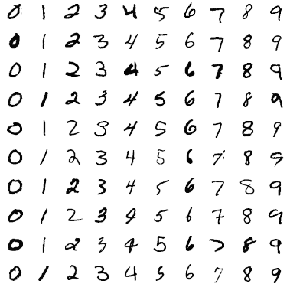
\includegraphics[width=5cm,height=5cm,keepaspectratio]{mnist_example.png}
  \centering
  \caption{MNIST Dataset Sample Images}
  \label{fig:mnist_sample}
\end{figure}
\end{frame}

\begin{frame}
\frametitle{Result Analysis}
\begin{center}
\begin{table}
\caption{Mean Accuracy}
\begin{tabular}{ || c c || } 
\hline
Artificial Neural Netwrok & Random Forest\\
\hline
0.875087508750875 & 0.9478947894789479\\
 \hline
\end{tabular}
\end{table}
\end{center}

\[
CM=
  \begin{bmatrix}
   965  &  0 &   1   & 1   & 1  &  2  &  3  &  1  &  5  &  0\\
0 & 1118  &  3  &  2  &  1   & 2  &  2  &  1 &   6 &   0\\
6  &  4 & 984 &   6  &  6  &  1  &  4 &  12  &  5  &  4\\
1  &  3  &  11  &  958  &  1  &  13  &  0  &  7 &   10  &   6\\
5  &   2 &   4  &  0 &  937 &   2 &   4  &  4 &   5 &  19\\
6   &  1  &   2  &  26  &  5  &  836  &  4   &  1  &   4 &   7\\
12  &  6  &  0 &   0  &  4 &  11 &  920  &   1  &  4  &  0\\
5   &  6 &  25  &   9  &  4  &  0  &  0 & 962  &  3 &  14\\
14  &  1 &  13 &  29 &  10 &  21 &   8 &   6 & 863 &    9
  \end{bmatrix}
\]
\centerline{Random Forest Confusion Matrix}

\end{frame}

\begin{frame}
\frametitle{Result Analysis}
\[
CM=
  \begin{bmatrix}
899  &  0  & 43  &  2  &  0 &  23  &  8  &  1  &  2  &  1\\
0 & 1096  &  2 &   2  &  0  &  1 &   1  &  1 &  30  &  2\\
13  &  3 & 857  &  3  &  8  & 43  & 25 &   7 &  53 &  20\\
1 &   5  &  9 & 900  &  0  & 55  &  0 &   7 &  33 &   0\\
0  &  0 &  10 &   0 & 875  &  0  & 19  &  4 &   5 &  69\\
21  &  4  & 52 & 142  &  0 & 626  &  5 &   0  & 38 &   4\\
18 &   1  & 38 &   0 &  20  &  3 & 871  &  0 &   5   & 2\\
1 &  31 &   3  &  1 &   2 &   0  &  1 & 924 &  19 &  46\\
4 &  14 &  37 &  18  &  6 &  13  &  0  &  7 & 860 &  15\\
1  &  6 &   8  &  5  &  66 &  14 &   2 &  40 &  25 & 842
  \end{bmatrix}
\]
\centerline{Confusion Matrix for Artificial Neural Network}
\end{frame}

\begin{frame}
\frametitle{Future Work}
\begin{itemize}
\item Improve hyper parameters
\item Try other variants of Neural Network (CNN, RNN etc)
\item Compare Other Classifiers
\end{itemize}

\end{frame}

\begin{frame}
\frametitle{Conclusion}

So from our we can say that Random Forest Classifier performed better than ANN. But there could be better hyper parameters for which ANN would outperform RF. 

\end{frame}

\end{document}
